
\section{Texture in Scene Images}

In computer graphics, texture mapping is a powerful tool which adds the surface detail to an object by wrapping
the color information from a digitized image. 
Texture is applied on top of a
polygon or 3D model to obtain a realistic rendering of it.
This makes rendering of objects more realistic than those without
surface texture. 
Scene images are extensively
used as source of textures as they are able to capture visual and structural information of the real world. They
are also able to capture a high level detail of object properties.
Generally an image is used as a texture map
on a planar surface. 

There are several texture mapping methods that avoids
modeling of the complex surface details. 
One of them is image-based rendering technique which is frequently used in computer graphics
in the form of texture mapping. The images are used to represent the appearance of a complex object.
It is a technique where images are used in place of complex geometry and material 
properties. Images are a quick way to achieve photorealism as our primary objective is to get 
a realistic rendering. This is because they are able to capture 
complex light interactions such as inter-reflections,
self-shadowing and sub-surface scattering present in the real world.
The main disadvantage of using images as rendering source is that the image captures the
appearance of the object from a single viewpoint and under a fixed lighting condition/direction. 
Therefore this method fails if the lighting conditions of the synthetic
environment are different from the lighting conditions of the texture image. This
is usually the case when we map 2D textures onto 3D models under varying lighting directions. 

\begin{figure*}[t]
\centering
\subfigure{
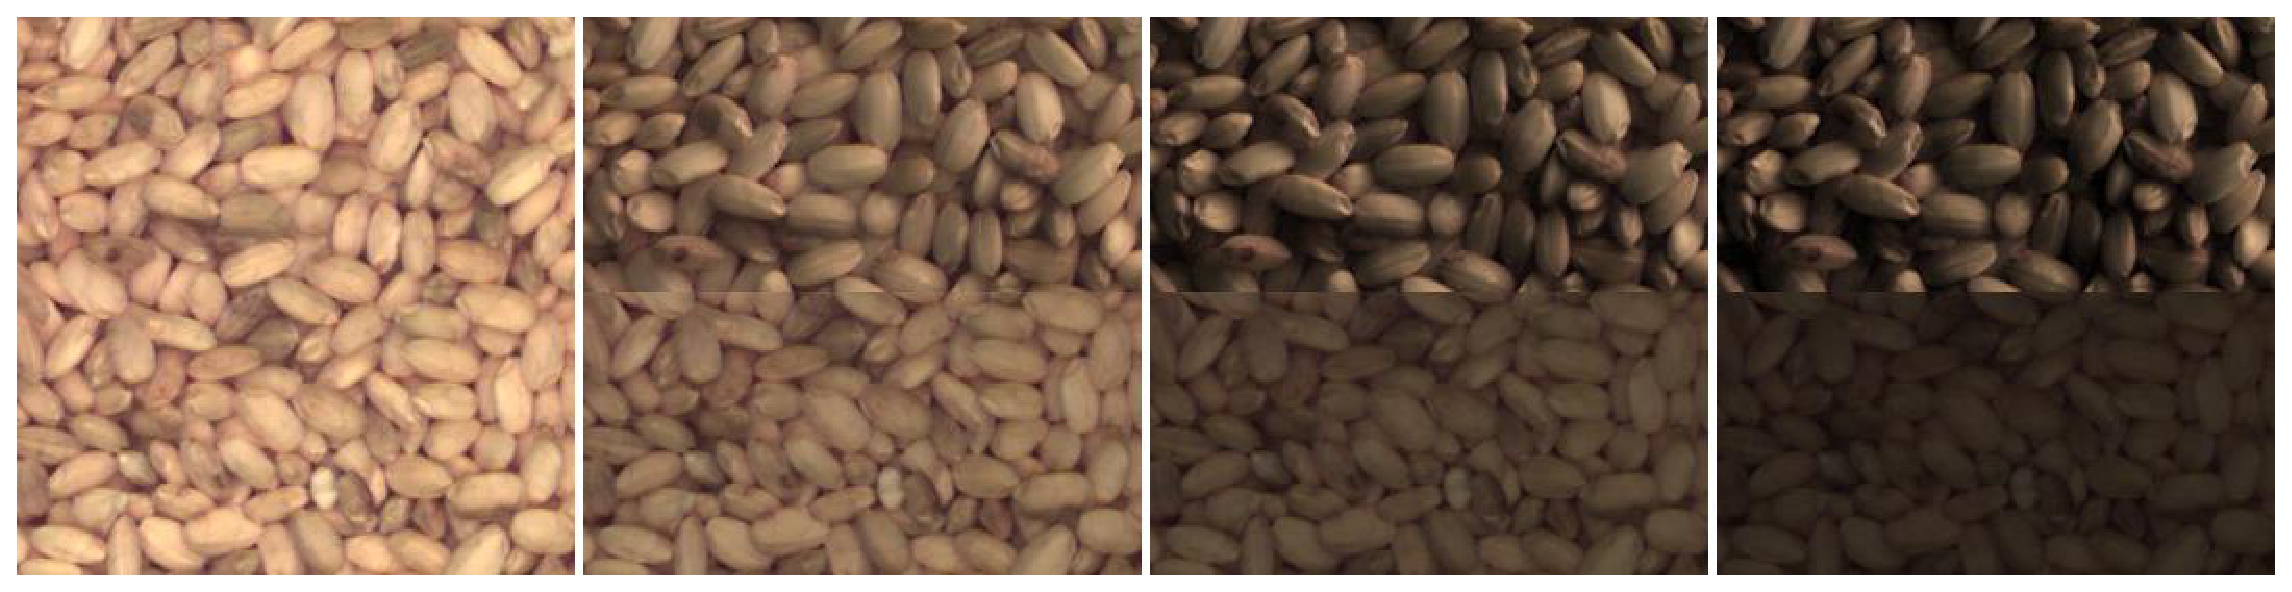
\includegraphics[scale=.4]{image_eps/ptm/ptm.eps}
\label{fig:subfig3} } \caption{3D vs 2D texture map:
The upper part of the images shows the visual appearance of
a 3D texture map while the bottom part shows the conventional 2D texture map. 
We can see that the bottom part suffers from unrealistic lighting and shadows.
} \label{fig:map}
\end{figure*}
In 2D texture modeling, the reflectance and the structural properties of natural surfaces
are not captured. They fail to capture the variations in surfaces for different lighting and
viewing directions. The texture which is mapped onto a 3D model has
the lighting direction from which it was captured. So if we want to see how the texture looks from
different lighting direction, this mapping will give poor results when viewed from different
lighting direction apart from the direction from which it was captured. In general, real world objects
are not flat and smooth in nature. They show different types of structural variation across their
surface each having different reflectance properties. These properties causes effects like shadows,
specularity, sub-surface scattering, inter-reflection etc. Hence 3D texture mapping
is required for realistic modeling of real objects.
It results in realistic rendering
of natural material surfaces. The characterization of surface reflectance properties is important in
achieving enhanced realism of the scene. The appearance of a surface in different lighting and viewing direction/
conditions is affected by its reflectance properties.
3D textures are a way to model the relation between surface reflectance
properties and illumination/viewing conditions. 
Fig \ref{fig:map} shows the difference between a 3D texture map and a 2D texture map.
To solve this
problem,
techniques based on reflectance texture maps have been proposed. 

Reflectance texture maps are one of
the techniques that can be used to compactly represent the 3D textures.
3D textures actually models the relation
between surface reflectance properties and illumination direction. Hence they can be represented
by Reflectance Texture Maps. The maps are generated using image re-lighting techniques
which model the surface reflectance properties of object. These
maps are created by capturing multiple images under different lighting/viewing conditions.

Reflectance map required in 3D texture can be modeled by Bidirectional Reflectance Distribution
Function (BRDF) \cite{chap2-22} technique which defines spectral and spatial reflectance characteristic of a
surface.
Bidirectional Reflectance Distribution Function is defined as the ratio of reflected radiance to
incident irradiance, given the lighting and viewing directions. 

Various techniques have been developed to compactly
represent BRDF \cite{chap2-18, chap2-19, chap2-20, chap2-21}
BRDF was extended to Bidirectional Texture Function (BTF) \cite{C2} by 
allowing BRDF to vary spatially
across planar texture co-ordinate (u,v).

BTF effectively captures view point dependent phenomenon such as specularity
along with other physical phenomenon such as shadow, sub-surface scattering,
inter-reflection, etc. However, the capture of BTF requires careful camera
calibration and capturing numerous images for sampling. Generating reflectance
map from BTF is very complex.
Because of the  high dimensionality of the BTF and high storage requirement,
Unidirectional Texture Functions (UTF) were introduced in which viewing point is
not taken into account while modeling the surface reflectance properties. They
model these properties only in relation to different lighting conditions. As the
visual appearance of the surface is mostly independent of the viewing direction,
the model provides a reasonable approximation of the surface with significantly
lower complexity of the model. Fig \ref{fig:model} shows the 3D texture modeling. 3D textures are mapped 
onto a 3D teapot model.

\begin{figure}[t]
\centering
\subfigure{
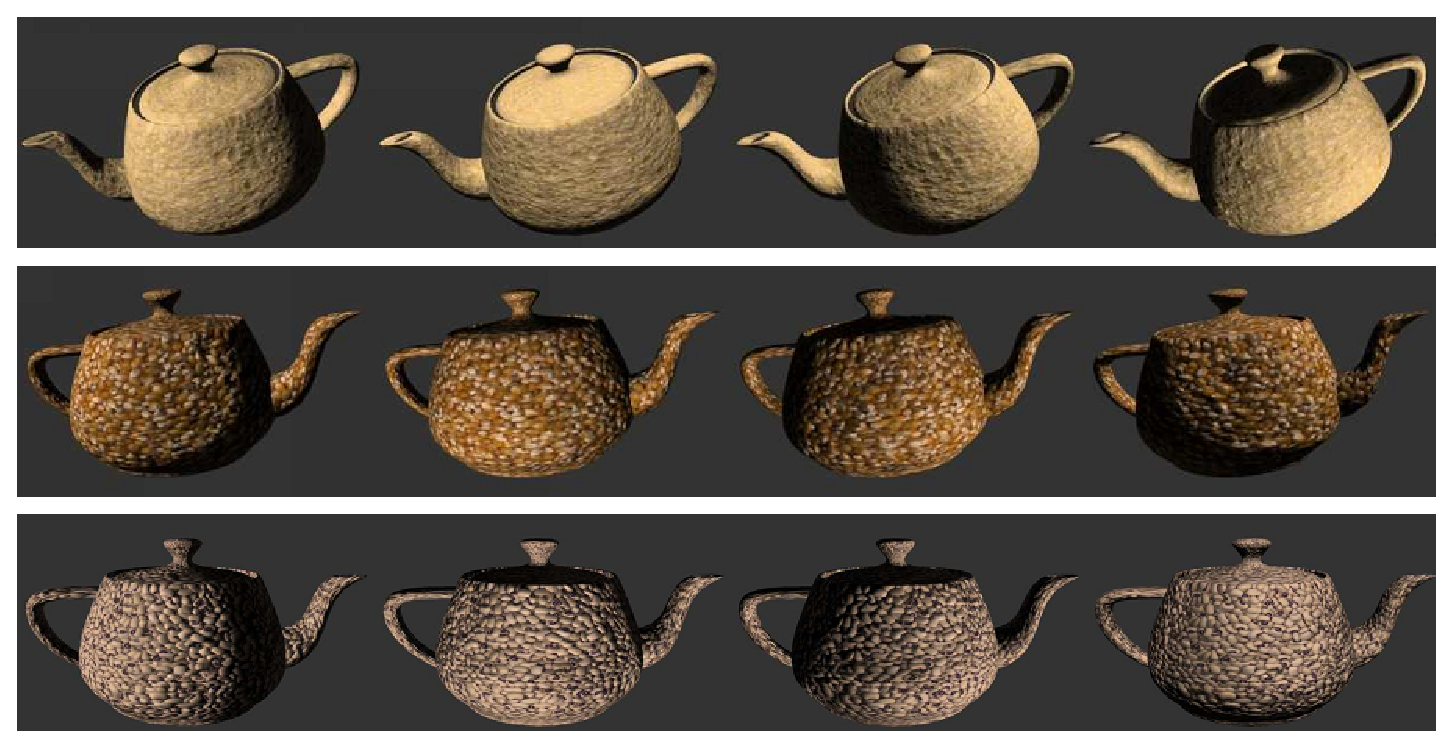
\includegraphics[height=4.2in,width=6in]{chap2/texture/res_1.eps}
}
\caption
{Natural textures mapped onto a 3D model of teapot under varying lighting directions}
\label{fig:model}
\end{figure}
Polynomial Texture Maps \cite{C4}
belong to the class of UTFs. It is a pixel
based technique that concisely models the surface reflectance properties using a
polynomial model for the reflectance, dependent on two angular parameters of the
lighting direction. 
It is used to model luminance
against changing lighting direction and requires
no modeling of complex geometry. Only a set of images is required of the desired scene to be used as a
texture which are taken from different known lighting
direction. PTMs reconstruct the color of the surface/texture under varying
lighting conditions and models real world phenomenon such as
self-shadowing, inter-reflection and sub-surface scattering.
When a surface is rendered with a PTM, it takes on different illumination
characteristics depending on the direction of the light source. They thus introduce
enhanced photorealism in the texture mapping process.

PTM model uses a set of input images captured from a fixed camera, where each
image is illuminated from a specific known lighting direction. It uses a
biquadratic polynomial function with 6 coefficients per pixel for modeling the
reflectance. These coefficients are estimated from the set of input images(30 to
40), where the lighting direction is resolved into two components i.e
$l_{u}$,$l_{v}$ by projecting it on the image plane. These two components are
used as variables in the biquadratic function. Once the coefficients are
estimated fitting the model to the observed values, they are used to render
images from any given lighting direction.
The function used in PTMs is:

\begin{equation}
L(l_u,l_v) = al_u^2 + bl_v^2 + cl_ul_v + dl_u + el_v +f
\end{equation}

But the PTM technique causes overall smoothening of light which dampens the effect
of specularity and softens sharp shadows. The effect of point light source is
reduced and the appearance is always similar to a diffused light source.  
The current state-of-the art in the field of PTM involves robust
method for interpolation of shadow and specularity, Drew {\em et al.} 
\cite{chap2-9}. But they do not model natural material surfaces and
their interactions with changing light conditions. Moreover
the number of per pixel parameters are too high for real-time
rendering

We improve upon the PTM model to overcome the above limitations
and generate a complete 3D Texture model that can be evaluated at individual
pixels. We propose an approach to image-based lighting interpolation that is
based on estimates of geometry and shading from a set of input images. We
decompose images captured at different lighting conditions into intrinsic image
components; i.e, the {\em direct} and {\em global} image components. Each of
these components is then further separated to obtain different physical
phenomena such as shadows, specularity and luminance. A final image is obtained
by combining the the individual models together.

\section{Text in Scene Images}

The aim of scene text localization and recognition is to find all areas in
an image that can be considered as text, mark
boundaries of the areas (rectangular bounding boxes) and output the word meanings of the detected content.
As the digital imaging devices are becoming cheaper and widely available, 
the size of the available digital image content is increasing rapidly.
The textual information present in images is very useful and needs to be extracted.
Therefore there is a growing demand to analyze, process and retrieve information
from multimedia content in an efficient way.
Some of the natural scene text images are shown in Fig \ref{fig:scene}.

\begin{figure}[t]
\centering
\subfigure{
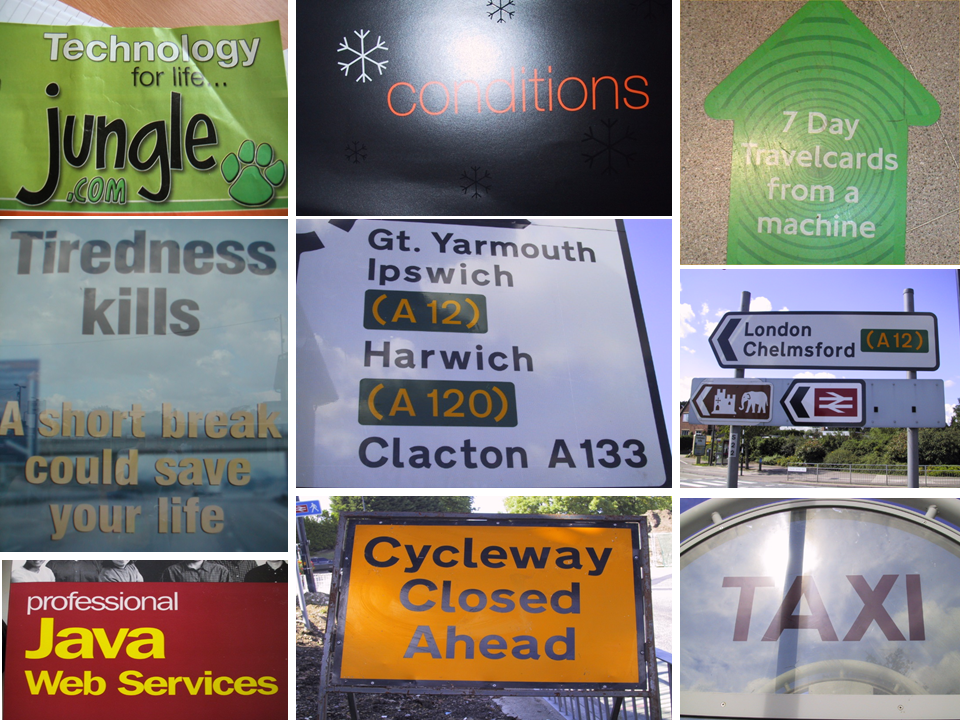
\includegraphics[height=4.3in,width=5.5in]{chap4/res_7/scene_images.eps}
}
\caption
{Some natural scenes containing text}
\label{fig:scene}
\end{figure}

\begin{figure}[t]
\centering
\subfigure{
\includegraphics[height=4.3in,width=5.5in]{chap4/res_7/text_pipe.eps}
}
\caption
{An end-to-end text recognition model}
\label{fig:textmodel}
\end{figure}

Recognizing text in scene images is a challenging task.
This is because the quality and content of images are
rather unpredictable. There are many variations in backgrounds (non-uniform), textures,
fonts and lighting conditions that are present in images.
To build a full end-to-end text recognition system, we need to develop models
which are robust to these variations. They should read all the text within the image and extract information. 
 
Most of the work on scene text recognition tends to focus on a sub-component of the
full end-to-end text recognition system.
The general problem of end-to-end text recognition
consists of three primary components:  

\begin{itemize}
 \item \textbf{Text detection:} Is there any text and where is it in the image? Locate it.
\item \textbf{Text Segmentation:} How to handle all the variations in background to extract 
foreground text as properly as possible.
\item \textbf{Text recognition:} What is the meaning of the word images?
\end{itemize}

In text
localization, the goal is to locate individual words or lines of text in the image.
The next step i.e text segmentation 
job is to extract the text properly so that it is better recognized afterwards. 
The extracted text goes to OCR for recognition.
Finally we identify the actual word meanings and
lines of the text. The recognized text is then used in various applications. 
An example of the end-to-end text recognition model is presented
in Fig \ref{fig:textmodel}


\begin{figure}[t]
\centering
\subfigure{
\includegraphics[height=4in,width=6in]{chap2/text_detect/results1.eps}
}
\caption
{Text detected in Scene Images}
\label{fig:detect}
\end{figure}


\begin{figure}[t]
\centering
\subfigure{
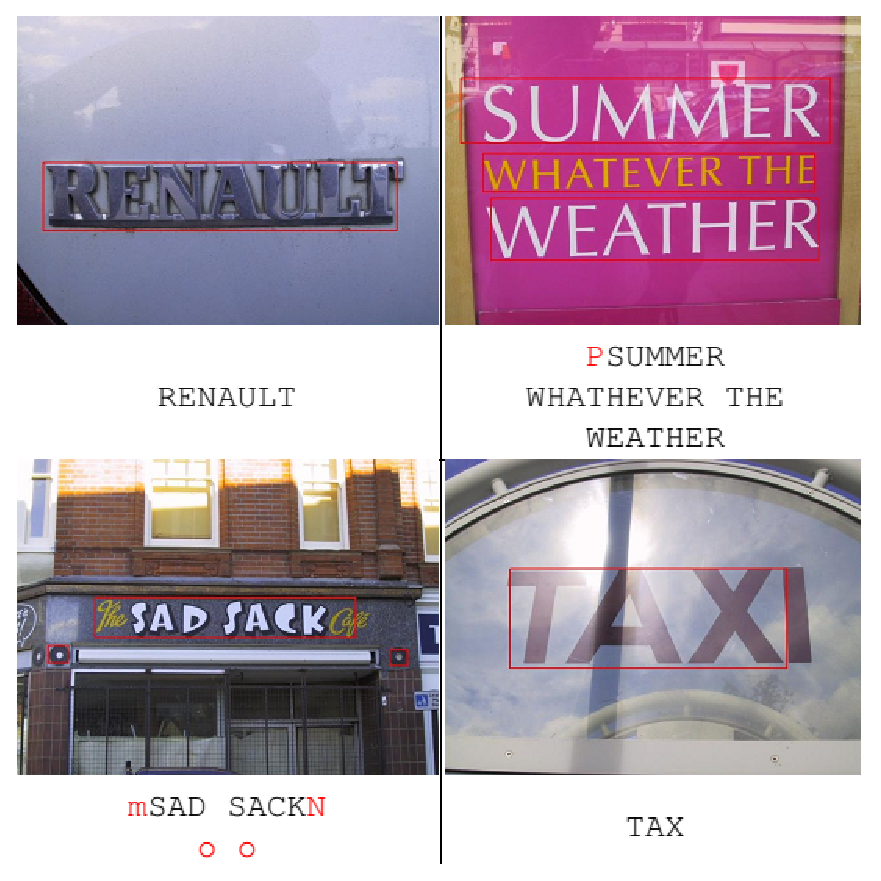
\includegraphics[height=3.6in,width=3in]{chap2/text_recog/res1.eps}
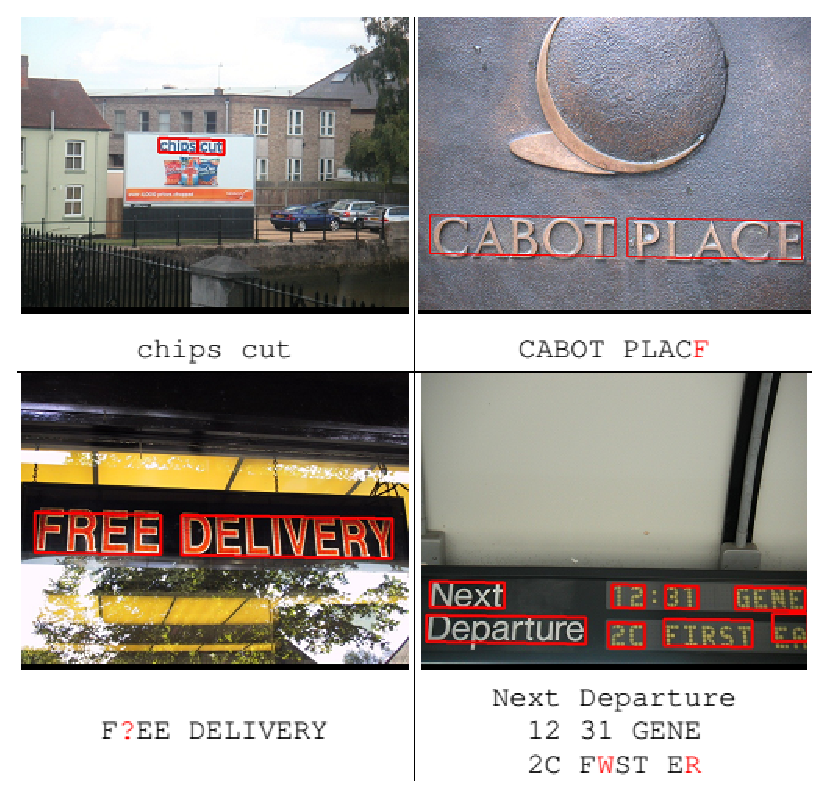
\includegraphics[height=3.6in,width=3in]{chap2/text_recog/res2.eps}
}
\caption
{Text recognized in Scene Images}
\label{fig:recog}
\end{figure}


\subsection{Text Detection and Recognition}

As mentioned above, the goal of text detection or localization is to identify regions
of text in a given scene image. The task of detection is 
to identify rectangle bounding box for each word or each line of text in the image.
There are methods which focus on general text localization problem.
It can be categorized into
two groups - (a) methods based on a sliding window and (b) methods based
on grouping of regions. 

Methods in the first group \cite{chap2-1, chap2-2, chap2-3}
%[4, 18, 15]
use a texture-based approach for text detection. A window is moved over the whole image and the position of text is
estimated on the basis of local image features. 
These methods are robust to noise.
But the computational complexity of these methods
is high because we need to search the text in image with many rectangles of different sizes and
aspect ratios. Also if the text is slanted or
perspectively distorted, then the sliding window methods do not produce
accurate text segmentation results.
Chen {\em et al.} \cite{chap2-1}
uses AdaBoost classifier having intensity variance features, histogram features,
mean intensity features, derivative features and edge linking features. 
They use a variant of Niblack's adaptive binarization algorithm for segmentation. 
The method is
computationally expensive. It also
requires manual segmentation of many sub-windows for training purposes and it seems
to over estimate the area of text in the image.
The above method was improved by Pan {\em et al.} \cite{chap2-2}
by adding a combination 
multi scale local binary pattern and histogram of gradient
features in the text detection stage. A Markov Random Field
(MRF) is used to group segmented characters into words. The method claims better localization
performance but it still suffers from high computational complexity.
Recently, Lee {\em et al.} \cite{chap2-3} further improved the approach by adding
more computationally expensive features which slightly improved the text localization performance
but it took longer time for processing.
Lienhart {\em et al.} \cite{chap2-4} uses a complex-valued multilayer feed-forward network 
which is trained to detect text at a fixed scale and position.
Coates {\em et al.} \cite{chap2-5} used unsupervised machine learning techniques
for character detection and recognition. A 32x32 pixel window is
shifted over the entire image in multiple scales and each patch is classified using a
linear SVM classifier as text or non-text. A variant of K-means method is used 
to generate features during training which are then used by the classifier.
However, the method does not provide end-to-end text recognition.

Recently published methods are based on the second category i.e region grouping 
\cite{chap2-7, chap2-8, chap2-10, chap2-11, chap2-12}.
In these methods, certain local features are computed for each pixel in the image and
then pixels with similar feature values are grouped together using connected
component analysis to form characters. 
But these methods are sensitive to noisy and low-resolution
images.
Ohya {\em et al.} \cite{chap2-6} was the first method which was based on character localization. 
In this method, they apply a local adaptive thresholding on grayscale 
images to detect candidate regions. The regions which have sufficient
contrast are termed as characters. Li {\em et al.} [16] \cite{chap2-13} apply thresholding in a
quantized color space. Then they group individual characters into text blocks
by some simple alignment rules. Both of the above methods assume that the 
background is uniform and characters are upright i.e
without any rotation. But this is not the case for general
text localization.
Kim {\em et al.}\cite{chap2-14} combine three independent detection channels i.e edge detection, 
color continuity and color variance
to find regions of possible text. These
regions are grouped into blocks by size and position. Each
block is divided into overlapping 16x16 pixel sub-blocks, which are
verified by a trained SVM classifier using wavelet transform to generate
features. The block is marked as text if the ratio of sub-blocks marked as text is higher than a pre-defined
threshold. The method is not scale-invariant as
the size of sub-blocks is constant.
Pan {\em et al.} \cite{chap2-7} 
uses a Waldboost classifier with histogram of gradient
as features. They create a text confidence map on a grayscale image pyramid.
Possible text regions are detected independently on a grayscale image using 
Niblack's binarization algorithm. A Conditional Random Field (CRF) is used
to label regions as
text or non-text.
To form block of texts, a simple gradient graph energy minimization approach is applied. 
Epshtein {\em et al.} \cite{chap2-11}
introduced an image operator: Stroke Width Transform (SWT). The SWT 
method uses Canny edge detector to find edges
and estimates stroke width for each pixel in the image.
A Connected component algorithm is then applied to form pixels with similar
stroke width into character candidates. These are merged into text blocks
using several heuristic rules. This method depends on the success of edge detection
which normally fails on noisy, blurred and low-contrast images.
Yao {\em et al.}\cite{chap2-8}
further improved this method. They replaced the
heuristic rules for character candidate detection and text block
formation by  trained classifiers with rotationally invariant features.
Fig \ref{fig:detect} shows text detected in scene images.

The methods listed above are focused only on text localization.
They estimate the location of the text but do not provide the contents meaning.
Mishra {\em et al.} \cite{chap2-12} proposed an effective method to recognize scene text. 
Their model combines bottom-up cues from
character detections and top-down cues from lexica.
Neumann and Matas \cite{chap2-10} proposed an end-to-end method for scene text localization and recognition.
They used hypotheses-verification
framework for processing multiple text line. They use 
synthetic fonts to train the algorithm thus eliminating the need for time consuming
acquisition and labeling of real-world training data. They also use
Maximally Stable Extremal Regions (MSER) which
are robust to geometric and lighting conditions.
A real time text localization and recognition was proposed by Neumann and Matas \cite{chap2-15}. 
This is achieved by posing the character detection problem as an efficient sequential selection 
from the set of Extremal Regions (ERs). The ER detector is robust to illumination, blur,
color and texture variation and also handles low-contrast text.
Neumann and Matas \cite{chap2-16} presented an unconstrained end-to-end text localization and recognition method.
The method introduces a novel
approach for character detection and recognition which
combines the advantages of sliding-window and connected
component methods. Fig \ref{fig:recog} shows text recognized in scene images.

\subsection{Text Segmentation}


\begin{figure*}[t]
\centering
\subfigure{

\includegraphics[height=.5in,width=1.1in]{chap4/threshold/res1/orig.eps}
}
\subfigure{

\includegraphics[height=.5in,width=1.1in]{chap4/threshold/res1/kit.eps}
}
\subfigure{

\includegraphics[height=.5in,width=1.1in]{chap4/threshold/res1/nib.eps}
}
\subfigure{

\includegraphics[height=.5in,width=1.1in]{chap4/threshold/res1/otsu.eps}
}
\subfigure{

\includegraphics[height=.5in,width=1.1in]{chap4/threshold/res1/sau.eps}
}
\subfigure{

\includegraphics[height=.5in,width=1.1in]{chap4/threshold/res2/orig.eps}
}
\subfigure{

\includegraphics[height=.5in,width=1.1in]{chap4/threshold/res2/kit.eps}
}
\subfigure{

\includegraphics[height=.5in,width=1.1in]{chap4/threshold/res2/nib.eps}
}
\subfigure{

\includegraphics[height=.5in,width=1.1in]{chap4/threshold/res2/otsu.eps}
}
\subfigure{

\includegraphics[height=.5in,width=1.1in]{chap4/threshold/res2/sau.eps}
}
\subfigure{

\includegraphics[height=.5in,width=1.1in]{chap4/threshold/res3/orig.eps}
}
\subfigure{

\includegraphics[height=.5in,width=1.1in]{chap4/threshold/res3/kit.eps}
}
\subfigure{

\includegraphics[height=.5in,width=1.1in]{chap4/threshold/res3/nib.eps}
}
\subfigure{

\includegraphics[height=.5in,width=1.1in]{chap4/threshold/res3/otsu.eps}
}
\subfigure{

\includegraphics[height=.5in,width=1.1in]{chap4/threshold/res3/sau.eps}
}
\subfigure{

\includegraphics[height=.5in,width=1.1in]{chap4/threshold/res4/orig.eps}
}
\subfigure{

\includegraphics[height=.5in,width=1.1in]{chap4/threshold/res4/kit.eps}
}
\subfigure{

\includegraphics[height=.5in,width=1.1in]{chap4/threshold/res4/nib.eps}
}
\subfigure{

\includegraphics[height=.5in,width=1.1in]{chap4/threshold/res4/otsu.eps}
}
\subfigure{

\includegraphics[height=.5in,width=1.1in]{chap4/threshold/res4/sau.eps}
}
\caption
{A comparison of scene text segmentation results.
From left to right (a) Text Image (b) kittler (c) Niblack (d) Otsu (e) Sauvola}
\label{fig:good}
\end{figure*}
The aim of text segmentation is to 
split an image into regions of foreground text and background.
If the text is extracted properly it can be better recognized afterwards.
OCR is able to recognize text if the input image is well formated and binarized.
Therefore we want to extract clean binary text images from complex backgrounds.

Thresholding is the basic method used for segmentation.
\cite{chap2-23} does a survey of thresholding based methods. Fig \ref{fig:good}
shows thresholding based binarization results. 
Recently, several methods for natural scene text binarization have been proposed.
Wakahara {\em et al.} \cite{chap2-24} proposes a technique which is composed of three parts:
They first generate tentative binarized images 
via dichotomization of k clusters obtained by k-means clustering in the HSI color space.
Then with the help of support vector machine (SVM), they determine
determine the degree of ``character-likeness'' of
each tentatively binarized image. Finally the binarized image having maximal degree
of ``character-likeness'' is selected as optimal binarization result.
To segment text information from camera-based images Thillou {\em et al.}
\cite{chap2-25} develops an automatic color thresholding method 
based on wavelet denoising and color clustering with K-means. 
Zhou {\em et al.} \cite{chap2-26} proposed a new text segmentation method based
on inverse rendering (decomposition of an input image into basic
rendering elements). The method uses iterative optimization to
solve the rendering parameters like material properties (for example diffuse/specular reflectance)
, blur kernel size and light source.
Field {\em et al.} \cite{chap2-27} describes
a novel technique for text segmentation that models smooth
color changes across image. They use bilateral regression technique for segmentation of
text from complex background.
Milyaev {\em et al.} \cite{chap4-4} proposed a new binarization method that works well for text in
natural scene images. The method embeds local binarization into
a global optimization framework. No information about the position and size of the text in an
image is required. It can also be used for text localization and for
recognition of the cropped text.
Mishra {\em et al.}~\cite{A16} has formulated the problem of binarization of text as an MRF optimization problem. 
The method shows superior performance over traditional binarization methods on many images and we use it as the
basis for our comparisons.

\section{Summary}
In this chapter, we introduced the problem of texture modeling.
We saw how scene images can be used as source of textures as they are able to
capture visual and structural information of the real world.
We showed the difference between the traditional 2D and 3D texture maps. 
We looked at how 2D textures results in unrealistic and incorrect rendering 
while 3D textures models the relation between surface
reflectance properties and illumination/viewing conditions thus resulting in realistic rendering.
We described the techniques like Bidirectional Reflectance Distribution
Function (BRDF) and Polynomial Texture Maps (PTM) used for modeling 3D textures.
We showed the disadvantages of using PTM model and how we propose to improve it.
We also looked into end-to-end text recognition model.
We saw how text detection helps in identifying regions of text in a
given scene image. A word recognizer then identifies the segmented words and finds
the underlying word meaning. We surveyed recent techniques applied to text detection, text segmentation 
and text recognition stages of the recognition model.
In the next chapter,
we propose a new framework where separation of images 
into {\em direct} and {\em global} components helps us in better modeling of 3D textures.
